\documentclass[aspectratio=169,11pt,t]{beamer}
% ============================================================
%  ksa-cs-v2: ksa-cs-lecture-template.tex 스타일 + 한글, v2 덱(16:9)용.
%    - 짙은 네이비 헤드라인 (섹션 이름 + 프레임마다 점)
%    - 꽉 찬 파란 제목 막대, 둥근 그림자 블록
%    - 한글: Noto Sans CJK KR (fontspec)
%  사용:
%    \documentclass[aspectratio=169,11pt,t]{beamer}
%    \input{<..>/theme/ksa-cs-v2.tex}
%  ksa-theme.tex 의 매크로(\kb \kq, ksablue/ksared 등)도 같은 이름으로 둔다
%  -> v2 덱 본문을 거의 그대로 옮길 수 있다.
% ============================================================

\usepackage{fontspec}
\usepackage{amsmath,amssymb}
\usepackage{tikz}
\usepackage{listings}
\usepackage{graphicx}
\usepackage{booktabs}
\usepackage{varwidth}
% enumitem 은 넣지 않는다 (beamer 글머리표가 사라진다)

\defaultfontfeatures{Ligatures=TeX}
\setmainfont{Noto Sans CJK KR}
\setsansfont{Noto Sans CJK KR}
\setmonofont{Noto Sans Mono CJK KR}[Scale=0.92]
\usefonttheme{professionalfonts}

% ---------- 기본 틀 ----------
\usetheme{default}
\useinnertheme[shadow=true]{rounded}
\setbeamertemplate{navigation symbols}{}
\setbeamersize{text margin left=1em,text margin right=1em}

% ---------- 색 (템플릿 원본 값) ----------
\definecolor{navydark}{HTML}{191959}
\definecolor{navydim}{HTML}{8888B0}
\definecolor{navytitle}{HTML}{262686}
\definecolor{navyblue}{HTML}{3333B2}
\definecolor{blockbodybg}{HTML}{E9E9F3}
\definecolor{examplegreen}{HTML}{006000}
\definecolor{examplebg}{HTML}{E5EFE5}
\definecolor{alertred}{HTML}{BF0000}
\definecolor{alertbg}{HTML}{F9E5E5}
% ksa-theme.tex 와 같은 이름 (본문 호환)
\colorlet{ksablue}{navytitle}
\colorlet{ksabluedk}{navydark}
\definecolor{ksagold}{HTML}{D6CBB1}
\definecolor{ksagolddk}{HTML}{A9976B}
\colorlet{ksared}{alertred}
\definecolor{ksagray}{HTML}{5B5B5B}

\setbeamercolor{structure}{fg=navyblue}
\setbeamercolor{alerted text}{fg=alertred}
\setbeamercolor{frametitle}{bg=navytitle,fg=white}
\setbeamercolor{title}{fg=white,bg=navytitle}
\setbeamercolor{block title}{bg=navytitle,fg=white}
\setbeamercolor{block body}{bg=blockbodybg,fg=black}
\setbeamercolor{block title example}{bg=examplegreen,fg=white}
\setbeamercolor{block body example}{bg=examplebg,fg=black}
\setbeamercolor{block title alerted}{bg=alertred,fg=white}
\setbeamercolor{block body alerted}{bg=alertbg,fg=black}
\setbeamercolor{item}{fg=navyblue}
\setbeamertemplate{itemize item}[circle]
\setbeamertemplate{itemize subitem}[triangle]

% ---------- 헤드라인: miniframes (섹션 이름 + 점) ----------
\useoutertheme[subsection=false]{miniframes}
\setbeamerfont{section in head/foot}{size=\tiny}
\setbeamercolor{section in head/foot}{bg=navydark,fg=white}
\setbeamercolor{mini frame}{fg=white}
\setbeamertemplate{mini frames}[circle]

% ---------- 제목 막대: 폭 꽉 채움, 두 줄까지 ----------
\setbeamerfont{frametitle}{size=\normalsize,series=\bfseries}
\setbeamertemplate{frametitle}{%
  \nointerlineskip
  \begin{beamercolorbox}[wd=\paperwidth,ht=2.7ex,dp=1.1ex,leftskip=.3cm,rightskip=.3cm]{frametitle}%
    \usebeamerfont{frametitle}\insertframetitle
  \end{beamercolorbox}}

% ---------- 쪽 번호: 오른쪽 아래 ----------
\setbeamertemplate{footline}{%
  \hfill
  {\color{navydim}\scriptsize\insertframenumber\,/\,\inserttotalframenumber}%
  \hspace{3mm}\vspace{2mm}%
}

% ---------- 표지: 템플릿처럼 헤드라인은 그대로, 가운데 둥근 그림자 상자에 제목 한 줄 ----------
% 덱에서:  {\setbeamertemplate{footline}{}\begin{frame}[c,noframenumbering]\titlepage\end{frame}}
\setbeamercolor{title}{fg=white,bg=navyblue}
\makeatletter
\setbeamertemplate{title page}{%
  \vfill
  \centering
  \begin{minipage}{0.84\paperwidth}
  \begin{beamercolorbox}[wd=\linewidth,sep=7pt,center,rounded=true,shadow=true]{title}
    {\usebeamerfont{title}\inserttitle\par}%
    \ifx\insertsubtitle\@empty\else\vskip0.4em{\usebeamerfont{subtitle}\insertsubtitle\par}\fi
  \end{beamercolorbox}
  \end{minipage}\par\vskip1.6em
  {\usebeamerfont{author}\color{navytitle}\insertauthor\par}\ifx\beamer@date\@empty\vskip0.3em\else\vskip1.3em\fi
  {\usebeamerfont{institute}\color{ksagray}\insertinstitute\par}%
  \ifx\beamer@date\@empty\else\vskip0.3em{\usebeamerfont{date}\color{ksagray}\insertdate\par}\fi
  \vfill
}
\makeatother
\setbeamerfont{title}{series=\bfseries,size=\Large}
\setbeamerfont{subtitle}{size=\normalsize}
\setbeamerfont{author}{size=\normalsize}
\setbeamerfont{institute}{size=\small}
\setbeamerfont{date}{size=\small}

% ksa-theme 호환: 덱이 \renewcommand{\ksacredit}{..} 를 해도 되게 (꼬리말에는 안 쓴다)
\newcommand{\ksacredit}{}

% ---------- 강조 ----------
\newcommand{\hl}[1]{\textcolor{alertred}{#1}}
\newcommand{\hlb}[1]{\textcolor{navyblue}{#1}}
\newcommand{\kb}[1]{\textbf{\color{ksablue}#1}}
\newcommand{\kq}[1]{\textbf{\color{ksared}#1}}

% ---------- 파이썬 코드 (템플릿과 같은 색) ----------
\definecolor{codekw}{HTML}{0033B3}
\definecolor{codebuiltin}{HTML}{BF0000}
\definecolor{codestr}{HTML}{067D17}
\definecolor{codecomment}{HTML}{8C8C8C}
\definecolor{codenum}{HTML}{1750EB}
\lstdefinestyle{py}{
  language=Python, basicstyle=\ttfamily\scriptsize,
  keywordstyle=\color{codekw}\bfseries, stringstyle=\color{codestr},
  commentstyle=\color{codecomment}\itshape, numberstyle=\color{codenum},
  emph={print,len,range,sum,input,int,str,float,list,dict,append,remove,sorted,abs,min,max},
  emphstyle=\color{codebuiltin}, showstringspaces=false, keepspaces=true,
  columns=fixed, basewidth=0.52em, aboveskip=1mm, belowskip=1mm, xleftmargin=2mm,
  breaklines=true
}
\lstset{style=py}

% ksa-cs-v2 색 바꾸기: 실험 덱 (주마다 3차시 실험, 보라)
% 사용: % ============================================================
%  ksa-cs-v2: ksa-cs-lecture-template.tex 스타일 + 한글, v2 덱(16:9)용.
%    - 짙은 네이비 헤드라인 (섹션 이름 + 프레임마다 점)
%    - 꽉 찬 파란 제목 막대, 둥근 그림자 블록
%    - 한글: Noto Sans CJK KR (fontspec)
%  사용:
%    \documentclass[aspectratio=169,11pt,t]{beamer}
%    \input{<..>/theme/ksa-cs-v2.tex}
%  ksa-theme.tex 의 매크로(\kb \kq, ksablue/ksared 등)도 같은 이름으로 둔다
%  -> v2 덱 본문을 거의 그대로 옮길 수 있다.
% ============================================================

\usepackage{fontspec}
\usepackage{amsmath,amssymb}
\usepackage{tikz}
\usepackage{listings}
\usepackage{graphicx}
\usepackage{booktabs}
\usepackage{varwidth}
% enumitem 은 넣지 않는다 (beamer 글머리표가 사라진다)

\defaultfontfeatures{Ligatures=TeX}
\setmainfont{Noto Sans CJK KR}
\setsansfont{Noto Sans CJK KR}
\setmonofont{Noto Sans Mono CJK KR}[Scale=0.92]
\usefonttheme{professionalfonts}

% ---------- 기본 틀 ----------
\usetheme{default}
\useinnertheme[shadow=true]{rounded}
\setbeamertemplate{navigation symbols}{}
\setbeamersize{text margin left=1em,text margin right=1em}

% ---------- 색 (템플릿 원본 값) ----------
\definecolor{navydark}{HTML}{191959}
\definecolor{navydim}{HTML}{8888B0}
\definecolor{navytitle}{HTML}{262686}
\definecolor{navyblue}{HTML}{3333B2}
\definecolor{blockbodybg}{HTML}{E9E9F3}
\definecolor{examplegreen}{HTML}{006000}
\definecolor{examplebg}{HTML}{E5EFE5}
\definecolor{alertred}{HTML}{BF0000}
\definecolor{alertbg}{HTML}{F9E5E5}
% ksa-theme.tex 와 같은 이름 (본문 호환)
\colorlet{ksablue}{navytitle}
\colorlet{ksabluedk}{navydark}
\definecolor{ksagold}{HTML}{D6CBB1}
\definecolor{ksagolddk}{HTML}{A9976B}
\colorlet{ksared}{alertred}
\definecolor{ksagray}{HTML}{5B5B5B}

\setbeamercolor{structure}{fg=navyblue}
\setbeamercolor{alerted text}{fg=alertred}
\setbeamercolor{frametitle}{bg=navytitle,fg=white}
\setbeamercolor{title}{fg=white,bg=navytitle}
\setbeamercolor{block title}{bg=navytitle,fg=white}
\setbeamercolor{block body}{bg=blockbodybg,fg=black}
\setbeamercolor{block title example}{bg=examplegreen,fg=white}
\setbeamercolor{block body example}{bg=examplebg,fg=black}
\setbeamercolor{block title alerted}{bg=alertred,fg=white}
\setbeamercolor{block body alerted}{bg=alertbg,fg=black}
\setbeamercolor{item}{fg=navyblue}
\setbeamertemplate{itemize item}[circle]
\setbeamertemplate{itemize subitem}[triangle]

% ---------- 헤드라인: miniframes (섹션 이름 + 점) ----------
\useoutertheme[subsection=false]{miniframes}
\setbeamerfont{section in head/foot}{size=\tiny}
\setbeamercolor{section in head/foot}{bg=navydark,fg=white}
\setbeamercolor{mini frame}{fg=white}
\setbeamertemplate{mini frames}[circle]

% ---------- 제목 막대: 폭 꽉 채움, 두 줄까지 ----------
\setbeamerfont{frametitle}{size=\normalsize,series=\bfseries}
\setbeamertemplate{frametitle}{%
  \nointerlineskip
  \begin{beamercolorbox}[wd=\paperwidth,ht=2.7ex,dp=1.1ex,leftskip=.3cm,rightskip=.3cm]{frametitle}%
    \usebeamerfont{frametitle}\insertframetitle
  \end{beamercolorbox}}

% ---------- 쪽 번호: 오른쪽 아래 ----------
\setbeamertemplate{footline}{%
  \hfill
  {\color{navydim}\scriptsize\insertframenumber\,/\,\inserttotalframenumber}%
  \hspace{3mm}\vspace{2mm}%
}

% ---------- 표지: 템플릿처럼 헤드라인은 그대로, 가운데 둥근 그림자 상자에 제목 한 줄 ----------
% 덱에서:  {\setbeamertemplate{footline}{}\begin{frame}[c,noframenumbering]\titlepage\end{frame}}
\setbeamercolor{title}{fg=white,bg=navyblue}
\makeatletter
\setbeamertemplate{title page}{%
  \vfill
  \centering
  \begin{minipage}{0.84\paperwidth}
  \begin{beamercolorbox}[wd=\linewidth,sep=7pt,center,rounded=true,shadow=true]{title}
    {\usebeamerfont{title}\inserttitle\par}%
    \ifx\insertsubtitle\@empty\else\vskip0.4em{\usebeamerfont{subtitle}\insertsubtitle\par}\fi
  \end{beamercolorbox}
  \end{minipage}\par\vskip1.6em
  {\usebeamerfont{author}\color{navytitle}\insertauthor\par}\ifx\beamer@date\@empty\vskip0.3em\else\vskip1.3em\fi
  {\usebeamerfont{institute}\color{ksagray}\insertinstitute\par}%
  \ifx\beamer@date\@empty\else\vskip0.3em{\usebeamerfont{date}\color{ksagray}\insertdate\par}\fi
  \vfill
}
\makeatother
\setbeamerfont{title}{series=\bfseries,size=\Large}
\setbeamerfont{subtitle}{size=\normalsize}
\setbeamerfont{author}{size=\normalsize}
\setbeamerfont{institute}{size=\small}
\setbeamerfont{date}{size=\small}

% ksa-theme 호환: 덱이 \renewcommand{\ksacredit}{..} 를 해도 되게 (꼬리말에는 안 쓴다)
\newcommand{\ksacredit}{}

% ---------- 강조 ----------
\newcommand{\hl}[1]{\textcolor{alertred}{#1}}
\newcommand{\hlb}[1]{\textcolor{navyblue}{#1}}
\newcommand{\kb}[1]{\textbf{\color{ksablue}#1}}
\newcommand{\kq}[1]{\textbf{\color{ksared}#1}}

% ---------- 파이썬 코드 (템플릿과 같은 색) ----------
\definecolor{codekw}{HTML}{0033B3}
\definecolor{codebuiltin}{HTML}{BF0000}
\definecolor{codestr}{HTML}{067D17}
\definecolor{codecomment}{HTML}{8C8C8C}
\definecolor{codenum}{HTML}{1750EB}
\lstdefinestyle{py}{
  language=Python, basicstyle=\ttfamily\scriptsize,
  keywordstyle=\color{codekw}\bfseries, stringstyle=\color{codestr},
  commentstyle=\color{codecomment}\itshape, numberstyle=\color{codenum},
  emph={print,len,range,sum,input,int,str,float,list,dict,append,remove,sorted,abs,min,max},
  emphstyle=\color{codebuiltin}, showstringspaces=false, keepspaces=true,
  columns=fixed, basewidth=0.52em, aboveskip=1mm, belowskip=1mm, xleftmargin=2mm,
  breaklines=true
}
\lstset{style=py}
 다음 줄에 % ksa-cs-v2 색 바꾸기: 실험 덱 (주마다 3차시 실험, 보라)
% 사용: % ============================================================
%  ksa-cs-v2: ksa-cs-lecture-template.tex 스타일 + 한글, v2 덱(16:9)용.
%    - 짙은 네이비 헤드라인 (섹션 이름 + 프레임마다 점)
%    - 꽉 찬 파란 제목 막대, 둥근 그림자 블록
%    - 한글: Noto Sans CJK KR (fontspec)
%  사용:
%    \documentclass[aspectratio=169,11pt,t]{beamer}
%    \input{<..>/theme/ksa-cs-v2.tex}
%  ksa-theme.tex 의 매크로(\kb \kq, ksablue/ksared 등)도 같은 이름으로 둔다
%  -> v2 덱 본문을 거의 그대로 옮길 수 있다.
% ============================================================

\usepackage{fontspec}
\usepackage{amsmath,amssymb}
\usepackage{tikz}
\usepackage{listings}
\usepackage{graphicx}
\usepackage{booktabs}
\usepackage{varwidth}
% enumitem 은 넣지 않는다 (beamer 글머리표가 사라진다)

\defaultfontfeatures{Ligatures=TeX}
\setmainfont{Noto Sans CJK KR}
\setsansfont{Noto Sans CJK KR}
\setmonofont{Noto Sans Mono CJK KR}[Scale=0.92]
\usefonttheme{professionalfonts}

% ---------- 기본 틀 ----------
\usetheme{default}
\useinnertheme[shadow=true]{rounded}
\setbeamertemplate{navigation symbols}{}
\setbeamersize{text margin left=1em,text margin right=1em}

% ---------- 색 (템플릿 원본 값) ----------
\definecolor{navydark}{HTML}{191959}
\definecolor{navydim}{HTML}{8888B0}
\definecolor{navytitle}{HTML}{262686}
\definecolor{navyblue}{HTML}{3333B2}
\definecolor{blockbodybg}{HTML}{E9E9F3}
\definecolor{examplegreen}{HTML}{006000}
\definecolor{examplebg}{HTML}{E5EFE5}
\definecolor{alertred}{HTML}{BF0000}
\definecolor{alertbg}{HTML}{F9E5E5}
% ksa-theme.tex 와 같은 이름 (본문 호환)
\colorlet{ksablue}{navytitle}
\colorlet{ksabluedk}{navydark}
\definecolor{ksagold}{HTML}{D6CBB1}
\definecolor{ksagolddk}{HTML}{A9976B}
\colorlet{ksared}{alertred}
\definecolor{ksagray}{HTML}{5B5B5B}

\setbeamercolor{structure}{fg=navyblue}
\setbeamercolor{alerted text}{fg=alertred}
\setbeamercolor{frametitle}{bg=navytitle,fg=white}
\setbeamercolor{title}{fg=white,bg=navytitle}
\setbeamercolor{block title}{bg=navytitle,fg=white}
\setbeamercolor{block body}{bg=blockbodybg,fg=black}
\setbeamercolor{block title example}{bg=examplegreen,fg=white}
\setbeamercolor{block body example}{bg=examplebg,fg=black}
\setbeamercolor{block title alerted}{bg=alertred,fg=white}
\setbeamercolor{block body alerted}{bg=alertbg,fg=black}
\setbeamercolor{item}{fg=navyblue}
\setbeamertemplate{itemize item}[circle]
\setbeamertemplate{itemize subitem}[triangle]

% ---------- 헤드라인: miniframes (섹션 이름 + 점) ----------
\useoutertheme[subsection=false]{miniframes}
\setbeamerfont{section in head/foot}{size=\tiny}
\setbeamercolor{section in head/foot}{bg=navydark,fg=white}
\setbeamercolor{mini frame}{fg=white}
\setbeamertemplate{mini frames}[circle]

% ---------- 제목 막대: 폭 꽉 채움, 두 줄까지 ----------
\setbeamerfont{frametitle}{size=\normalsize,series=\bfseries}
\setbeamertemplate{frametitle}{%
  \nointerlineskip
  \begin{beamercolorbox}[wd=\paperwidth,ht=2.7ex,dp=1.1ex,leftskip=.3cm,rightskip=.3cm]{frametitle}%
    \usebeamerfont{frametitle}\insertframetitle
  \end{beamercolorbox}}

% ---------- 쪽 번호: 오른쪽 아래 ----------
\setbeamertemplate{footline}{%
  \hfill
  {\color{navydim}\scriptsize\insertframenumber\,/\,\inserttotalframenumber}%
  \hspace{3mm}\vspace{2mm}%
}

% ---------- 표지: 템플릿처럼 헤드라인은 그대로, 가운데 둥근 그림자 상자에 제목 한 줄 ----------
% 덱에서:  {\setbeamertemplate{footline}{}\begin{frame}[c,noframenumbering]\titlepage\end{frame}}
\setbeamercolor{title}{fg=white,bg=navyblue}
\makeatletter
\setbeamertemplate{title page}{%
  \vfill
  \centering
  \begin{minipage}{0.84\paperwidth}
  \begin{beamercolorbox}[wd=\linewidth,sep=7pt,center,rounded=true,shadow=true]{title}
    {\usebeamerfont{title}\inserttitle\par}%
    \ifx\insertsubtitle\@empty\else\vskip0.4em{\usebeamerfont{subtitle}\insertsubtitle\par}\fi
  \end{beamercolorbox}
  \end{minipage}\par\vskip1.6em
  {\usebeamerfont{author}\color{navytitle}\insertauthor\par}\ifx\beamer@date\@empty\vskip0.3em\else\vskip1.3em\fi
  {\usebeamerfont{institute}\color{ksagray}\insertinstitute\par}%
  \ifx\beamer@date\@empty\else\vskip0.3em{\usebeamerfont{date}\color{ksagray}\insertdate\par}\fi
  \vfill
}
\makeatother
\setbeamerfont{title}{series=\bfseries,size=\Large}
\setbeamerfont{subtitle}{size=\normalsize}
\setbeamerfont{author}{size=\normalsize}
\setbeamerfont{institute}{size=\small}
\setbeamerfont{date}{size=\small}

% ksa-theme 호환: 덱이 \renewcommand{\ksacredit}{..} 를 해도 되게 (꼬리말에는 안 쓴다)
\newcommand{\ksacredit}{}

% ---------- 강조 ----------
\newcommand{\hl}[1]{\textcolor{alertred}{#1}}
\newcommand{\hlb}[1]{\textcolor{navyblue}{#1}}
\newcommand{\kb}[1]{\textbf{\color{ksablue}#1}}
\newcommand{\kq}[1]{\textbf{\color{ksared}#1}}

% ---------- 파이썬 코드 (템플릿과 같은 색) ----------
\definecolor{codekw}{HTML}{0033B3}
\definecolor{codebuiltin}{HTML}{BF0000}
\definecolor{codestr}{HTML}{067D17}
\definecolor{codecomment}{HTML}{8C8C8C}
\definecolor{codenum}{HTML}{1750EB}
\lstdefinestyle{py}{
  language=Python, basicstyle=\ttfamily\scriptsize,
  keywordstyle=\color{codekw}\bfseries, stringstyle=\color{codestr},
  commentstyle=\color{codecomment}\itshape, numberstyle=\color{codenum},
  emph={print,len,range,sum,input,int,str,float,list,dict,append,remove,sorted,abs,min,max},
  emphstyle=\color{codebuiltin}, showstringspaces=false, keepspaces=true,
  columns=fixed, basewidth=0.52em, aboveskip=1mm, belowskip=1mm, xleftmargin=2mm,
  breaklines=true
}
\lstset{style=py}
 다음 줄에 % ksa-cs-v2 색 바꾸기: 실험 덱 (주마다 3차시 실험, 보라)
% 사용: \input{../../../theme/ksa-cs-v2.tex} 다음 줄에 \input{../../../theme/ksa-cs-v2-lab.tex}
% 수업 덱은 기본 파란색 그대로. 공용 테마 파일은 건드리지 않는다.
\definecolor{navytitle}{HTML}{4B2380}
\definecolor{navydark}{HTML}{2A1350}
\definecolor{navyblue}{HTML}{6A3DA8}
\definecolor{navydim}{HTML}{B3A2CF}
\definecolor{blockbodybg}{HTML}{EFEAF6}
\colorlet{ksablue}{navytitle}
\colorlet{ksabluedk}{navydark}

% 수업 덱은 기본 파란색 그대로. 공용 테마 파일은 건드리지 않는다.
\definecolor{navytitle}{HTML}{4B2380}
\definecolor{navydark}{HTML}{2A1350}
\definecolor{navyblue}{HTML}{6A3DA8}
\definecolor{navydim}{HTML}{B3A2CF}
\definecolor{blockbodybg}{HTML}{EFEAF6}
\colorlet{ksablue}{navytitle}
\colorlet{ksabluedk}{navydark}

% 수업 덱은 기본 파란색 그대로. 공용 테마 파일은 건드리지 않는다.
\definecolor{navytitle}{HTML}{4B2380}
\definecolor{navydark}{HTML}{2A1350}
\definecolor{navyblue}{HTML}{6A3DA8}
\definecolor{navydim}{HTML}{B3A2CF}
\definecolor{blockbodybg}{HTML}{EFEAF6}
\colorlet{ksablue}{navytitle}
\colorlet{ksabluedk}{navydark}

% 2주차 3차시 실험. 옛 강의 덱 (3주차 03-1) 은 _이전/overfitting_lecture.tex
\setbeamerfont{author}{size=\normalsize}
\setbeamerfont{institute}{size=\small}
\graphicspath{{figs/}{../../../assets/}}
\usepackage{booktabs}
\makeatletter
\newcommand{\markpage}[1]{\protected@write\@auxout{}{\string\newlabel{#1}{{\the\c@framenumber}{}}}\hypertarget{#1}{}}
\newcommand{\pref}[1]{\hyperlink{#1}{\textcolor{ksagolddk}{(p.\ref{#1})}}}
\makeatother

\renewcommand{\ksacredit}{Machine Learning and Deep Learning \,\textperiodcentered\, 실험: 과대적합과 과소적합}
\title{실험: 곡선을 복잡하게 하면 예측이 좋아질까?}
\subtitle{과대적합 · 과소적합 · 교차 검증을 직접 찾아내기}
\author{Machine Learning and Deep Learning}
\institute{KSA 2027-Spring}
\date{Sumin Han (suminhan@ksa.hs.kr)}
\begin{document}
{\setbeamertemplate{footline}{}\begin{frame}[c,noframenumbering]\titlepage\end{frame}}

\section{질문}
% --- 오늘의 실험 질문
\begin{frame}{오늘의 실험 질문}
\vfill
\centering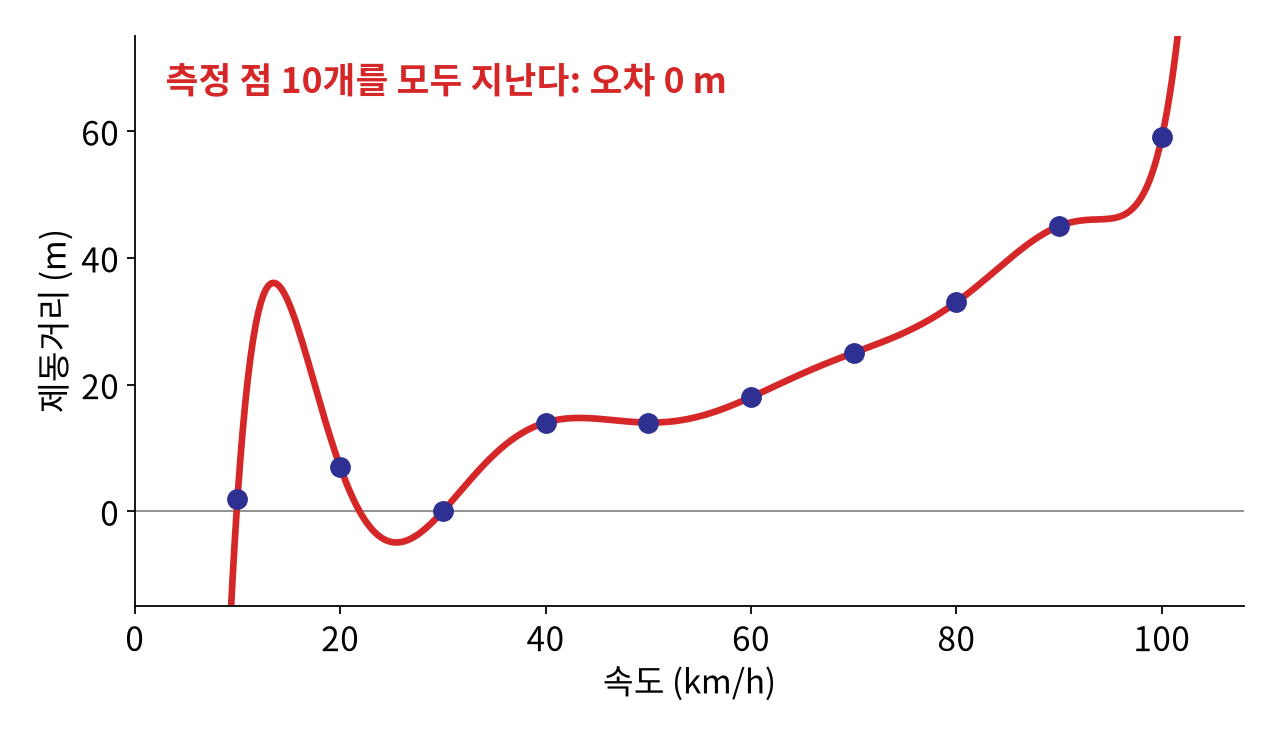
\includegraphics[width=0.58\linewidth]{of_hook.png}\par\vskip0.3em
{\large 측정한 점을 모두 지나는 곡선. \kq{이 모델이 처음 보는 속도의 제동거리도 잘 맞힐까?}}\par\vskip0.3em
{\small 오늘은 강의 대신 실험으로 답을 찾습니다. 결과는 표 하나와 해석 한 문단으로 냅니다.}
\vfill
\note{오늘 3차시는 실험 시간입니다. 1차시에 선형회귀로 직선을 그었고, 오늘은 곡선을 점점 복잡하게 만들어 봅니다. 화면의 빨간 곡선은 측정한 점 10개를 하나도 빠짐없이 지나갑니다. 측정 데이터에서는 오차가 0입니다. 그러면 이 모델이 처음 보는 속도의 제동거리도 잘 맞힐까요? 오늘은 제가 답을 알려 주지 않고, 여러분이 실험으로 찾습니다. 끝나면 결과 표 하나와 해석 한 문단을 냅니다.}
\end{frame}

% --- 데이터
\begin{frame}{실험 재료: 제동거리 데이터}
\markpage{data}
\vfill
\centering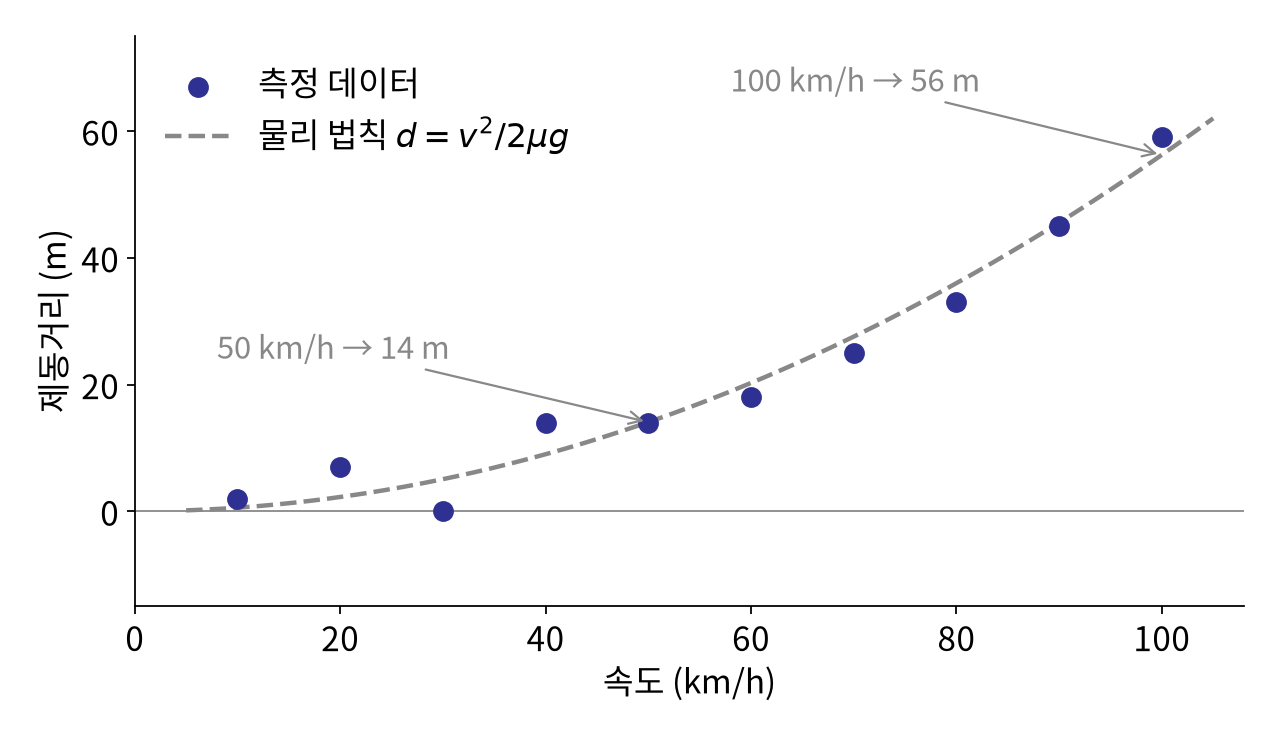
\includegraphics[width=0.55\linewidth]{of_data.png}\par\vskip0.2em
{\large 측정 데이터 \kb{10개}로 모델을 만들고, 나중에 잰 \kq{새 데이터 6개}로 시험합니다}\\[0.3em]
{\small 제동거리 = 브레이크를 밟고 멈출 때까지 간 거리. 점은 물리 법칙 $d = v^2/(2\mu g)$ 에 측정 오차를 더한 예시입니다.}
\vfill
\note{실험 재료는 자동차 제동거리입니다. 속도를 바꿔 가며 10번 잰 측정 데이터가 있고, 모델을 다 만든 뒤에 새로 잰 데이터 6개가 따로 있습니다. 측정 데이터로 모델을 만들고, 새 데이터로 시험합니다. 회색 점선은 물리 법칙인데, 오늘은 이 법칙을 모른다고 치고 점만 보고 모델을 고릅니다. 30킬로에서 0미터처럼 이상한 점도 있는데, 실제 측정에도 이런 잡음은 늘 섞입니다.}
\end{frame}

% --- 가설
\begin{frame}{실험 전에: 가설을 먼저 적습니다}
\markpage{hypo}
\vfill
\centering
{\Large 직선(1차) · 2차 곡선 · 9차 곡선 중\\[0.3em] \kb{새 데이터를 가장 잘 맞힐 모델}은?}\par\vskip1.2em
\begin{tabular}{ll}
\toprule
\textbf{적을 것} & \textbf{예시 형식} \\
\midrule
고른 모델 & ``9차 곡선'' \\
이유 한 줄 & ``측정 오차가 가장 작으니까'' \\
\bottomrule
\end{tabular}\par\vskip1em
{\small 노트북 맨 위 ``가설'' 칸에 적습니다. 틀려도 감점 없습니다. \kq{실험 후에 고치지 마세요.}}
\vfill
\note{실험을 시작하기 전에 가설을 먼저 적습니다. 직선, 2차 곡선, 9차 곡선 중 새 데이터를 가장 잘 맞힐 모델은 무엇일까요? 고른 모델과 이유 한 줄을 노트북 맨 위 가설 칸에 적으세요. 틀려도 감점은 없습니다. 다만 실험 후에 고치면 안 됩니다. 가설과 결과가 다를 때 왜 달랐는지를 쓰는 게 오늘 해석 문단의 핵심입니다. 논문도 이렇게 씁니다.}
\end{frame}

% --- 절차
\begin{frame}{실험 절차 (50분)}
\vfill
\centering
\renewcommand{\arraystretch}{1.5}
\begin{tabular}{clp{8.4cm}}
\toprule
& \textbf{실험} & \textbf{할 일} \\
\midrule
\kb{1} & 차수 올리기 {\small (15분)} & 1차부터 9차까지 맞추고, 측정 데이터 오차와 새 데이터 오차를 \kb{표}에 적는다 \\
\kb{2} & 새 데이터 없이 고르기 {\small (15분)} & 새 데이터가 아직 없다고 치고, \kb{5겹 교차 검증}으로 차수를 고른다 \\
\kb{3} & 실제 자동차 50대 {\small (15분)} & 1920년대에 잰 진짜 데이터에서 같은 방법으로 차수를 고른다 \\
& 해석 쓰기 {\small (5분)} & 결과 표 + 해석 한 문단 \pref{report} \\
\bottomrule
\end{tabular}\par\vskip0.8em
{\small 오차는 평균 절대 오차 \quad $\text{MAE} = \frac{1}{m}\sum_{i=1}^{m}\big|h(x^{(i)}) - y^{(i)}\big|$ \quad (단위: m)}
\vfill
\note{실험은 세 개입니다. 실험 1에서는 다항식 차수를 1차부터 9차까지 올리면서 측정 데이터 오차와 새 데이터 오차를 표에 적습니다. 실험 2에서는 새 데이터가 아직 없다고 치고, 측정 데이터만으로 차수를 고르는 방법을 해 봅니다. 실험 3에서는 1920년대에 실제로 잰 자동차 50대 데이터에서 같은 방법으로 차수를 고릅니다. 마지막 5분은 해석을 씁니다. 오차는 평균 절대 오차로 잽니다. 예측과 실제의 차이에 절댓값을 씌워 평균 낸 값이라, 단위가 미터 그대로입니다.}
\end{frame}

% --- 기록표
\begin{frame}{실험 1 \& 2: 이 표를 채웁니다}
\markpage{table}
\vfill
\centering
{\Large\renewcommand{\arraystretch}{1.4}\begin{tabular}{lccc}
\toprule
\textbf{차수} & \textbf{측정 데이터 오차} & \textbf{새 데이터 오차} & \textbf{교차 검증 오차} \\
\midrule
1 (직선) & \underline{\hspace{1.4cm}} & \underline{\hspace{1.4cm}} & \underline{\hspace{1.4cm}} \\
2 & \underline{\hspace{1.4cm}} & \underline{\hspace{1.4cm}} & \underline{\hspace{1.4cm}} \\
3 & \underline{\hspace{1.4cm}} & \underline{\hspace{1.4cm}} & \underline{\hspace{1.4cm}} \\
9 & \underline{\hspace{1.4cm}} & \underline{\hspace{1.4cm}} & \underline{\hspace{1.4cm}} \\
\bottomrule
\end{tabular}}\par\vskip1em
{\large 실험 1이 끝나면 스스로 물어보세요: \kb{측정 데이터에서 1등인 모델이 새 데이터에서도 1등인가?}}
\vfill
\note{실험 1과 2에서 채울 표입니다. 노트북은 1차부터 9차까지 전부 출력하지만, 표에는 1, 2, 3, 9차만 옮겨 적습니다. 실험 1이 끝나면 측정 데이터 오차에서 1등인 모델과 새 데이터 오차에서 1등인 모델이 같은지 확인해 보세요. 같지 않다면, 왜 다른지가 오늘의 핵심 질문입니다.}
\end{frame}

% --- 교차 검증 방법
\begin{frame}{실험 2의 방법: 5겹 교차 검증}
\markpage{cv}
\vfill
\centering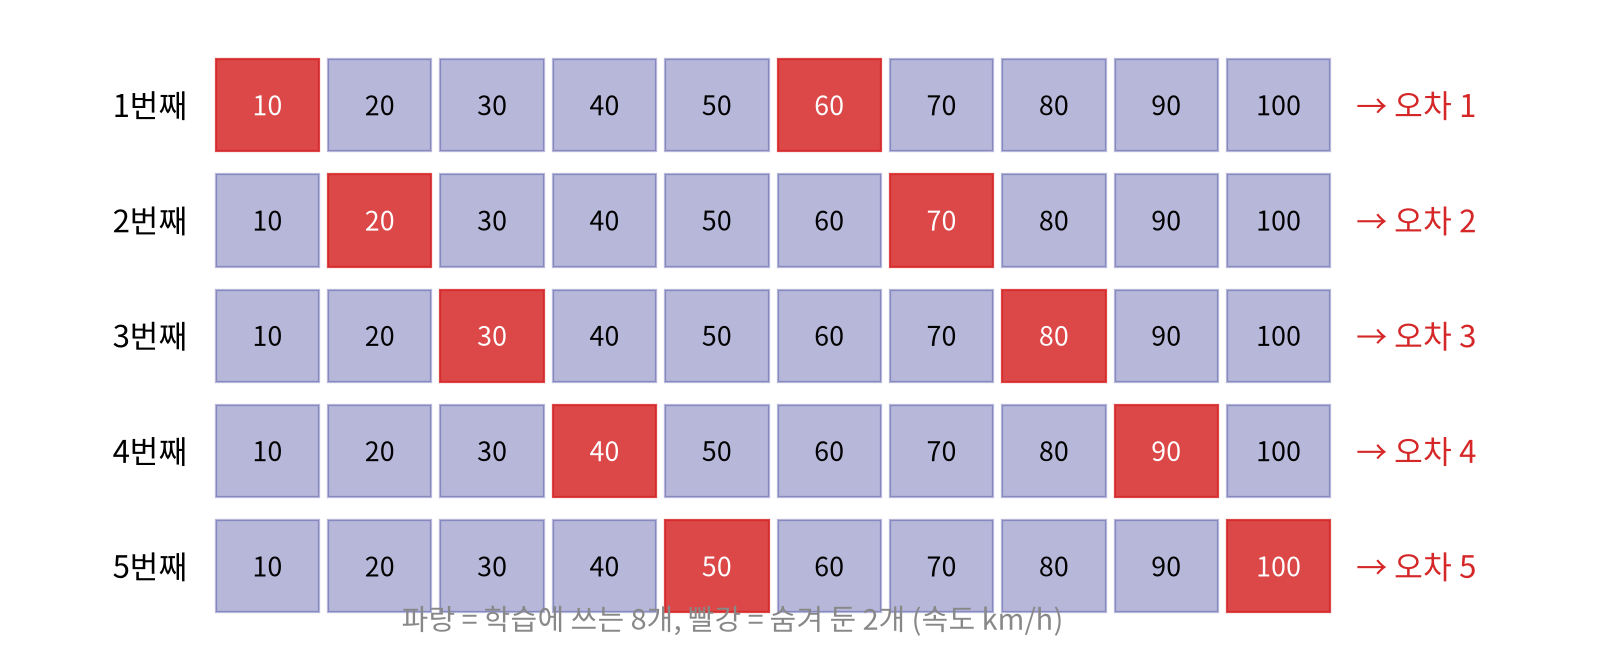
\includegraphics[width=0.52\linewidth]{of_folds.png}\par\vskip0.1em
{\large 새 데이터가 없으면 \kb{가진 데이터 일부를 숨겨 두고} 숨긴 것으로 시험합니다}\\[0.3em]
{\small 점 10개 $\to$ 2개씩 5조각. 한 조각을 숨기고 8개로 학습 $\to$ 숨긴 2개의 오차. 다섯 번 돌아가며 평균 \quad $\text{CV} = \frac{1}{5}\sum_{k=1}^{5}\text{MAE}_k$}
\vfill
\note{실험 2의 방법입니다. 실제로 모델을 고를 때는 새 데이터가 아직 없습니다. 미래의 데이터니까요. 그래서 가진 데이터 일부를 숨겨 두고, 나머지로 학습한 다음 숨긴 데이터로 시험합니다. 점이 10개뿐이라 한 번만 숨기면 운에 따라 결과가 크게 바뀌니까, 2개씩 5조각으로 나눠서 돌아가며 숨깁니다. 다섯 번의 오차 평균이 교차 검증 오차입니다. 노트북에서 이 반복문의 빈칸 두 줄을 채우면 됩니다. 교차 검증 오차가 실험 1의 새 데이터 오차와 비슷한 모양을 그리는지 보세요.}
\end{frame}

% --- 제출
\begin{frame}{제출: 결과 표 + 해석 한 문단}
\markpage{report}
\vfill
\centering
\begin{tabular}{p{4.0cm}p{9.0cm}}
\toprule
\textbf{해석 문단에 들어갈 것} & \textbf{예시 문장의 틀} \\
\midrule
가설과 결과 비교 & ``우리는 ○○를 예상했지만, 새 데이터에서는 ○○가 가장 좋았다 (○.○ m).'' \\
왜 그런지 & ``○차 곡선은 측정 데이터 오차가 ○ m 인데 새 데이터에서는 ○ m 였다. 그 이유는 ...'' \\
교차 검증이 고른 것 & ``새 데이터 없이 교차 검증만으로도 ○차를 골랐다.'' \\
실제 데이터 & ``자동차 50대에서는 ○차를 골랐고, 이는 물리 법칙과 (맞는다 / 다르다).'' \\
\bottomrule
\end{tabular}\par\vskip0.8em
{\small 노트북 맨 아래 ``결과와 해석'' 칸에 쓰고 제출합니다. 숫자는 반드시 \kb{직접 실행한 결과}를 씁니다.}
\vfill
\note{제출물은 결과 표와 해석 한 문단입니다. 해석 문단에는 네 가지가 들어갑니다. 가설과 결과를 비교하고, 왜 그런 결과가 나왔는지 쓰고, 교차 검증이 무엇을 골랐는지, 실제 자동차 데이터에서는 어땠는지. 화면의 틀을 그대로 써도 됩니다. 숫자는 반드시 직접 실행한 결과를 씁니다. 이게 프로젝트 보고서의 결과와 분석 절을 아주 작게 연습하는 것입니다.}
\end{frame}

\section{실험 후}
% --- 실험 후: 이름 붙이기
\begin{frame}{실험이 끝난 뒤: 여러분이 본 것의 이름}
\vfill
\centering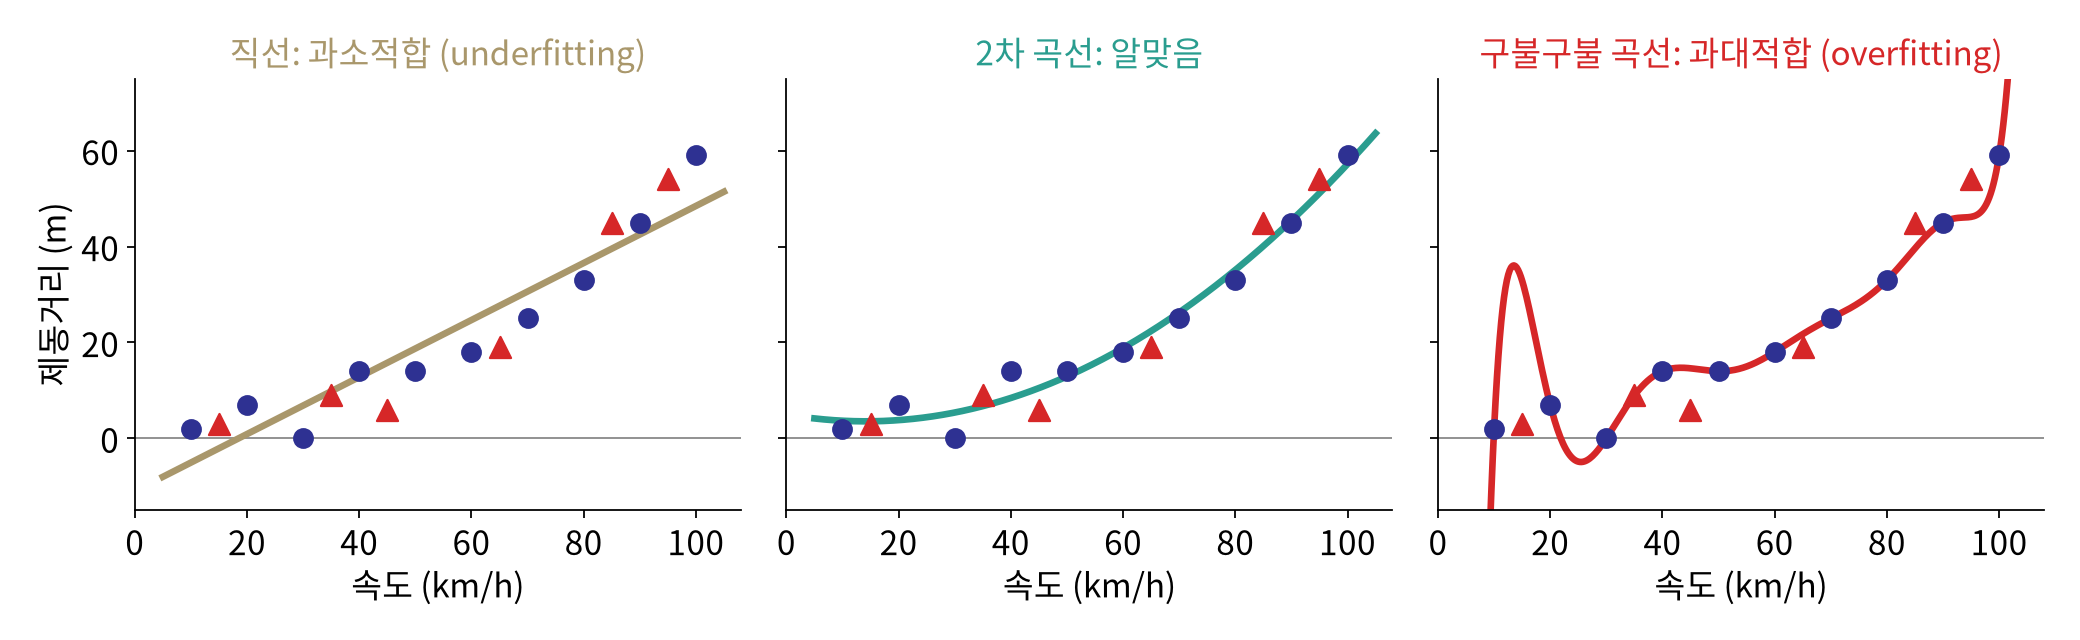
\includegraphics[width=0.92\linewidth]{of_three.png}\par\vskip0.3em
{\large \kb{과소적합}: 너무 단순해서 가진 데이터도 못 따라간다 \qquad \kq{과대적합}: 가진 데이터를 외워서 새 데이터를 틀린다}
\vfill
\note{실험이 끝난 뒤에 보여 주는 쪽입니다. 여러분이 표에서 본 것에 이름을 붙입니다. 직선은 측정 데이터 오차도 새 데이터 오차도 둘 다 컸습니다. 너무 단순해서 가진 데이터조차 못 따라간 것이고, 이걸 과소적합이라고 합니다. 9차 곡선은 측정 데이터 오차가 0인데 새 데이터 오차가 컸습니다. 측정한 점을 외워 버린 것이고, 이걸 과대적합이라고 합니다. 가운데 2차 곡선이 그 사이의 알맞은 복잡도입니다.}
\end{frame}

% --- U자
\begin{frame}{실험 후: 차수를 1부터 9까지 놓고 보면}
\vfill
\centering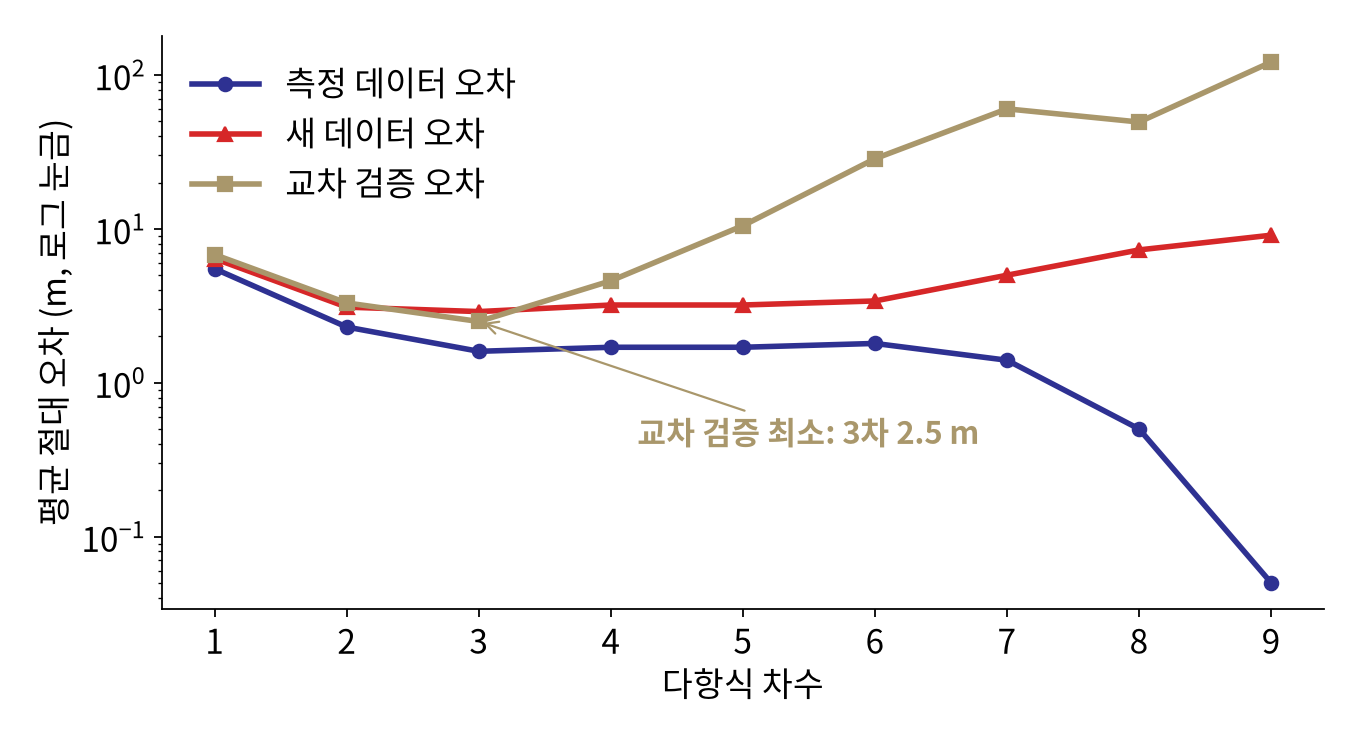
\includegraphics[width=0.58\linewidth]{of_sweep.png}\par\vskip0.3em
{\large 측정 오차는 계속 줄지만, 교차 검증 오차는 \kb{U자}: 2차 3.3 m · 3차 2.5 m 에서 바닥}\\[0.2em]
{\small 둘이 비슷하면 단순한 쪽을 고른다 \quad (9차의 측정 오차 0 m 는 로그 눈금이라 바닥에 붙여 그렸다)}
\vfill
\note{1차부터 9차까지 한 그래프에 모았습니다. 측정 데이터 오차는 차수를 올릴수록 계속 줄어서 9차에서 0이 됩니다. 반면 교차 검증 오차는 U자 모양이고, 3차가 2.5미터, 2차가 3.3미터로 바닥입니다. 점이 10개뿐이라 이 정도 차이는 잡음 수준이고, 비슷하면 더 단순한 2차를 고르는 게 보통입니다. 실제 물리 법칙도 2차입니다. 새 데이터 오차도 같은 U자를 그립니다. 교차 검증이 새 데이터 오차를 잘 흉내 낸다는 뜻입니다. 학습에 쓴 데이터의 오차로는 모델을 고를 수 없다, 이게 오늘의 결론입니다.}
\end{frame}

% --- 9차를 넘어
\begin{frame}{더 생각해 볼 것: 9차를 넘어 계속 키우면?}
\vfill
\centering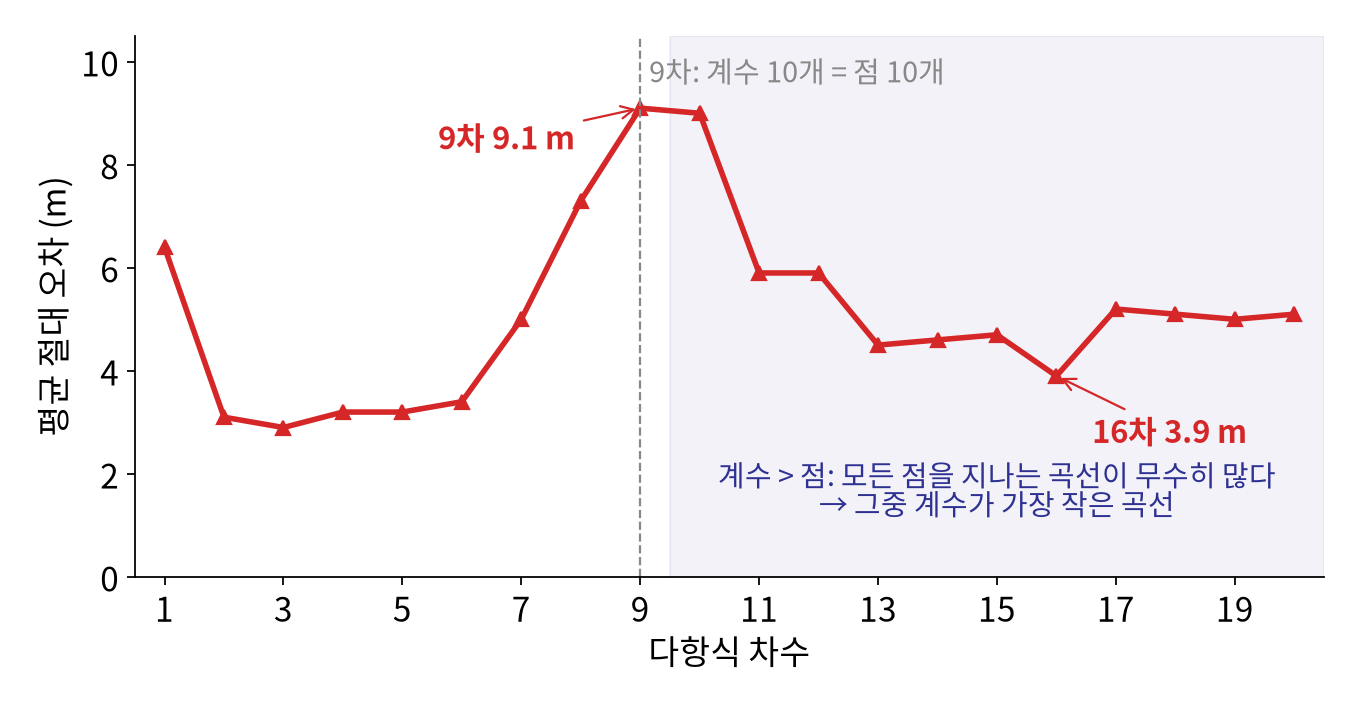
\includegraphics[width=0.56\linewidth]{of_beyond.png}\par\vskip0.3em
{\large 9차 \kq{9.1 m} 에서 끝이 아니다: 계수가 점보다 많아지자 \kb{다시 내려간다} (16차 \kb{3.9 m})}\\[0.2em]
{\small 10차부터 측정 오차는 모두 0 m \quad 3차 2.9 m 보다는 못하다 \quad $\to$ 15주차 \textbf{이중 하강 (double descent)}}
\vfill
\note{질문 하나를 남깁니다. 9차가 새 데이터에서 9.1미터로 가장 나빴으니 더 키우면 더 나빠질까요? 실제로 해 보면 그렇지 않습니다. 10차부터는 계수가 점보다 많아서 모든 점을 지나는 곡선이 무수히 많고, 그중 계수가 가장 작은 곡선을 고르면 새 데이터 오차가 16차에서 3.9미터까지 다시 내려갑니다. 이걸 이중 하강이라고 부르고, 15주차에 큰 신경망과 함께 다시 다룹니다.}
\end{frame}

% --- 정리
\begin{frame}{정리}
\vfill
\centering\large\begin{tabular}{l}
\kb{과소적합} \quad 너무 단순해서 가진 데이터도 못 따라간다 (두 오차 모두 큼)\\[0.5em]
\kq{과대적합} \quad 가진 데이터를 외워서 새 데이터를 틀린다 (측정 오차만 작음)\\[0.5em]
학습에 쓴 데이터의 오차로는 모델을 고를 수 없다\\[0.5em]
\textbf{교차 검증} \quad 돌아가며 숨겨 두고 맞혀 본 오차의 평균으로 고른다
\end{tabular}\par\vskip1em
{\normalsize\href{https://colab.research.google.com/github/SuminHan/book-ml/blob/main/slides/ml1/week02/3_overfitting/lab/overfitting.ipynb}{\textcolor{ksagolddk}{▶ Colab에서 실험 노트북 열기}} \quad {\small 데이터: 제동거리 예시 · cars (Ezekiel, 1930; R 기본 데이터)}}
\vfill
\note{정리합니다. 과소적합은 너무 단순해서 가진 데이터도 못 따라가는 것, 과대적합은 가진 데이터를 외워서 새 데이터를 틀리는 것입니다. 학습에 쓴 데이터의 오차는 외울수록 작아지니까 모델을 고르는 기준이 될 수 없고, 그래서 교차 검증으로 고릅니다. 5주차에 정규화와 함께 교차 검증을 다시 자세히 다룹니다.}
\end{frame}
\end{document}
